\documentclass[11pt,a4paper]{article}
\usepackage[T1]{fontenc}
\usepackage[utf8]{inputenc}
\usepackage{lmodern,amsmath,amssymb,booktabs,longtable,graphicx,geometry,xurl,hyperref,microtype}
\geometry{margin=25mm}
\hypersetup{colorlinks=true,urlcolor=blue,citecolor=blue,linkcolor=blue}
\renewcommand{\topfraction}{0.9}
\renewcommand{\textfraction}{0.08}
\renewcommand{\floatpagefraction}{0.85}
\newcommand{\doctype}{Technical report}
\newcommand{\docversion}{0.01.000}
\newcommand{\docdate}{1 November 2026}
\newcommand{\versiondoi}{10.5281/zenodo.23851660}
\newcommand{\conceptdoi}{10.5281/zenodo.23851659}
\newcommand{\docrepo}{github.com/fsantibanezleal/CAOS\_SoftQP}
\newcommand{\headerblock}{\begin{center}\fbox{\parbox{0.94\textwidth}{\small\raggedright
\textbf{\doctype}\quad v\docversion, \docdate\quad Licence CC BY 4.0\\[3pt]
CAOS Research\quad Soft-constrained optimization\\[3pt]
Version DOI: \texttt{\versiondoi}\\
Concept DOI (always latest): \texttt{\conceptdoi}\\[3pt]
Not peer reviewed. Source code, data and computational records:\\
\href{https://\docrepo}{\texttt{\docrepo}}
}}\end{center}}
\title{Side-Specific Soft Constraints in Quadratic Programming}
\author{Felipe Santibáñez-Leal\\\small ORCID: \href{https://orcid.org/0000-0002-0150-3246}{0000-0002-0150-3246}}
\date{}
\begin{document}
\maketitle
\headerblock
\begin{abstract}
Soft constraints in control and energy optimization represent priced departures from selected operating limits. Their interpretation depends on which rows remain hard, which interval side is violated and whether the price is linear, quadratic or coupled across rows. We implement separable side-specific linear--quadratic interval costs in a native OSQP-style projection path and compare equivalent formulations through independent lifting, the published generalized slack projection implementation, DAQP, a fixed-parameter FlexQP reconstruction and ElastiQP. Fifteen synthetic or source-faithful cases cover scalar semantics, mixed hard/soft rows, grouped penalties, semidefinite curvature, control conflict and a building-energy model. A preregistered computation comprises 456 seeded instances and seven measured repetitions, retaining 11592 accepted observations and 7560 incompatible cells without numerical or accuracy-rejected observations. The primary paired relative cold end-to-end reduction against the faster matched baseline is 0.50\%, with a 95\% seed-cluster interval of $[-3.29\%,3.94\%]$, so the predicted 10\% improvement is not established. A separate 32-frame common-trajectory control example distinguishes warm-state reuse from hard-constraint safety. The results support numerical equivalence within the tested families, while showing that unchanged principal dimensions alone do not establish an end-to-end advantage or algorithmic novelty.
\end{abstract}

\section{Problem and operating context}
Quadratic programs frequently combine immutable physical limits with preferences that may yield. In model predictive control, actuator capacity and model equations can remain hard while selected comfort or state targets incur a cost. In energy scheduling, a temperature departure, a battery-health departure and a contracted grid overage have different physical units and consequences. A single undifferentiated label ``soft'' is therefore insufficient to specify the optimization problem.

The engineering policy precedes the numerical algorithm. Assigning a finite cost to a row permits departure when its benefit elsewhere exceeds its price. A mathematically optimal elastic solution can violate an original operational inequality. Conversely, an infeasible hard model cannot be repaired merely by reporting a successful status for a different relaxed objective. Physical safety, model adequacy and numerical optimality are distinct questions.

We study transparent synthetic models rather than field performance. Scalar inputs isolate sign conventions. Sparse instances vary numerical structure. A condensed double integrator isolates recovery under bounded actuation. A published two-zone building model supplies a coupled energy example with mixed penalties. Its two separable variants deliberately change the objective, so their resulting policies are not reproductions of the mixed-penalty optimum.

\section{Related work and comparison boundary}
OSQP solves convex quadratic programs by operator splitting and provides warm starts, sparse linear-system preparation and numerical infeasibility checks \cite{osqp}. Generalized slack projections extend soft-constraint handling through proximal operations without necessarily increasing the principal QP dimensions \cite{gsp}. The published implementation supports symmetric separable penalties and selected grouped or Huber costs. Its unconditional-penalty assumptions are more specific than arbitrary asymmetric convex costs.

DAQP already exposes separate lower/upper linear and quadratic soft weights \cite{daqp}. Consequently, unequal side costs are not a new modeling capability. A comparison restricted to a symmetric default would confound a policy change with an algorithmic difference. The DAQP adapter used here preserves original-scale prices, maps its reciprocal quadratic convention and refuses unsupported objectives rather than adding a small regularizer.

FlexQP and Deep FlexQP address elastic optimization through a splitting formulation and, for the learned variant, a trained numerical-parameter policy \cite{flex}. We independently reconstruct the fixed equations and Algorithm~1, not the authors' implementation or trained policy. ElastiQP supplies a separate published dual active-set backend for compatible linear elastic inequalities \cite{elasti}. A finite L1 price can purchase violation; exact recovery of a feasible hard optimum requires sufficiently large weights relative to appropriate optimal multipliers.

Active-set reuse and reduced-system correction are also established ideas. qpOASES exploits parametric QP structure \cite{qpoases}, and OSQP polishing guesses an active set before solving an additional linear system \cite{osqp}. Neither an active-set guess nor a subsequent KKT check alone establishes a new method. No global priority claim is made for asymmetric proximal handling, fixed-size representations or elastic feasibility.

\section{Original-space formulation}
Let $P\succeq0$, $q\in\mathbb R^n$, $A\in\mathbb R^{m\times n}$ and $\ell_i\le u_i$, allowing a missing interval side. For $z=Ax$, define
\begin{equation}
v_{\ell,i}=(\ell_i-z_i)_+,\qquad v_{u,i}=(z_i-u_i)_+ .
\end{equation}
For soft rows $i\in S$, choose finite nonnegative side coefficients $a_{\ell,i},a_{u,i},b_{\ell,i},b_{u,i}$. The objective is
\begin{align}
F(x)&=\tfrac12x^\top Px+q^\top x+\sum_{i\in S}g_i(A_ix),\\
g_i(z)&=a_{\ell,i}(\ell_i-z)_++a_{u,i}(z-u_i)_+
 +\tfrac12b_{\ell,i}(\ell_i-z)_+^2+\tfrac12b_{u,i}(z-u_i)_+^2 .
\end{align}
Rows outside $S$ satisfy $\ell_i\le A_ix\le u_i$ as hard constraints. In an extended-real formulation, their $g_i$ is the interval indicator. A missing side contributes no penalty. Equality rows require the same side conventions at their common endpoint.

Each scalar soft cost is proper, closed and convex for the stated coefficients and a nonempty interval. Its derivative is nondecreasing on each exterior branch and joins the zero interior derivative through an admissible subgradient interval. Strict convexity of $P$ is sufficient for uniqueness when a minimizer exists, but semidefinite curvature alone does not imply existence or uniqueness. Hard infeasibility and unbounded directions remain possible in the general model.

The signed slack convention is $s_i=v_{\ell,i}-v_{u,i}$: an upper overshoot has negative recovered slack. Physical violation plots retain lower and upper nonnegative quantities instead of allowing signed cancellation. A sum of raw meters, degrees and kilowatt-hours has no physical interpretation without a separately defined normalization or cost.

\subsection{Explicit lifting}
An ordinary lift introduces nonnegative finite-side variables and imposes
\begin{equation}
A_ix+t_{\ell,i}\ge\ell_i,\qquad A_ix-t_{u,i}\le u_i,
\qquad t_{\ell,i},t_{u,i}\ge0,
\end{equation}
with the corresponding linear--quadratic costs. Hard rows receive no such relaxation. Symmetric costs use the authors' compact signed/shared-slack construction when applicable; forcing all symmetric cases into a larger general lift would create an unnecessarily weak baseline.

The lift is an independent representation of the original objective, not a change in its policy. Recovered original variables and duals are evaluated outside the backend. High-accuracy stock OSQP supplies the independent numerical oracle. Timed ordinary lifting instead uses the same native fork as the projection path, separating formulation effects from differences between OSQP builds.

\subsection{Side-specific interval proximal operation}
For a scalar temporary value $v$ and $\rho>0$, consider
\begin{equation}
\operatorname{prox}_{g_i/\rho}(v)
 =\arg\min_z\left[g_i(z)+\tfrac\rho2(z-v)^2\right].
\end{equation}
For a soft row, the unique minimizer is
\begin{equation}
\operatorname{prox}_{g_i/\rho}(v)=
\begin{cases}
\ell_i-\dfrac{\bigl(\rho(\ell_i-v)-a_{\ell,i}\bigr)_+}{\rho+b_{\ell,i}},&v<\ell_i,\\[8pt]
v,&\ell_i\le v\le u_i,\\[4pt]
u_i+\dfrac{\bigl(\rho(v-u_i)-a_{u,i}\bigr)_+}{\rho+b_{u,i}},&v>u_i.
\end{cases}
\label{eq:prox}
\end{equation}
The missing-side branch is omitted. A hard row uses interval projection.

\paragraph{Derivation.}
Inside the interval, both $g_i$ and the squared displacement are minimized at $z=v$. Above the upper endpoint, differentiating the smooth exterior branch gives $(\rho+b_{u,i})(z-u_i)=\rho(v-u_i)-a_{u,i}$. If the right side is nonpositive, the minimizer is the endpoint; otherwise it gives the stated exterior displacement. The lower case follows by reversing the signed displacement and using lower-side coefficients. Strong convexity of the proximal subproblem and the endpoint subgradient conditions establish uniqueness. This argument is a scalar convex minimization, not a novelty claim.

\subsection{Operator splitting and convergence scope}
Writing the problem as $\min_{x,z}f(x)+g(z)$ subject to $Ax=z$ yields the usual two-block splitting. The side coefficients enter the proximal operation rather than enlarging the principal quadratic system. With fixed numerical parameters, its linear-system dimensions retain the original variables and constraint rows. Adaptive changes of numerical $\rho$ can still require refactorization; unchanged dimensions are not a promise of one factorization forever.

Convergence is conditional on the assumptions required by the underlying convex splitting method, including an appropriate primal--dual solution. The scalar derivation does not prove arbitrary adaptive-parameter behavior, every implementation-level scaling rule, or every numerical infeasibility certificate. The source tests cover concrete bounded/unbounded and hard-infeasible examples, but finite test coverage is not a general theorem for all such instances.

\section{Optimality and semantic verification}
Original-space stationarity is
\begin{equation}
Px+q+A^\top y=0.
\end{equation}
It must be accompanied by $y\in\partial g(Ax)$ and hard feasibility. The fixed-point condition
\begin{equation}
z=\operatorname{prox}_{g}(z+y),\qquad z=Ax,
\label{eq:kkt}
\end{equation}
tests the subgradient relation with a unit diagnostic proximal scale, independently of the solver's numerical ADMM parameter. At a kink it avoids selecting an arbitrary derivative. A stationary unconstrained target outside a priced interval can have zero gradient balance with $y=0$ while failing Eq.~\eqref{eq:kkt}.

Upper-side lifted multipliers enter the original dual positively and lower-side multipliers negatively. Equality multipliers retain their row positions. The evaluator recomputes base objective, side penalty, original lower/upper violations and maximum hard error. Semantically incompatible objectives are not assigned a zero error or an empty successful result.

Backend statuses have distinct meanings. DAQP's status two denotes a soft optimum; OSQP's status two denotes an inaccurate solution. The external timing-study acceptance requires a successful method-specific status, normalized objective discrepancy
\begin{equation}
\delta_F=\frac{|F(x)-F(x_{\rm oracle})|}{\max(1,|F(x_{\rm oracle})|)}\le10^{-6}
\end{equation}
and maximum raw hard-row violation at most $10^{-6}$. Stationarity is diagnostic in that preregistered computation. Full primal/dual vectors remain available in the catalog and control examples; the repeated timing JSONL stores scalar diagnostics rather than every solution vector.

\section{Implemented comparison paths}
\begin{longtable}{p{0.18\textwidth}p{0.37\textwidth}p{0.37\textwidth}}
\toprule Method & Compared objective & Important boundary\\\midrule
Ordinary lifting & Symmetric compact or separate-side separable costs; exact helpers for mixed published examples & Independent stock oracle; matched native backend for timed lift\\
Generalized projection & Published symmetric separable, Huber and selected grouped costs & Unequal side coefficients are incompatible\\
Asymmetric projection & Separable nonnegative side-specific linear--quadratic costs & CPU builtin path; no asymmetric grouped or Huber extension\\
DAQP & Positive-definite elastic objectives with positive quadratic price on every finite soft side & Reciprocal quadratic convention; no inserted regularizer or L1 substitution\\
FlexQP reconstruction & Positive finite-side L1 soft inequalities & Fixed paper equations; no finite hard rows, quadratic soft costs or trained policy\\
ElastiQP 0.2.0 & Positive-definite pure L1 inequalities and hard equalities & Hard inequalities and quadratic side costs refused\\\bottomrule
\end{longtable}

The FlexQP reconstruction uses $\sigma_x=10^{-6}$, $\sigma_s=1$, $\rho=1$ and relaxation $\alpha=1.6$. Its Schur system is
\begin{equation}
K=P+\sigma_x I+cG^\top G,\qquad c=(\sigma_s^{-1}+\rho^{-1})^{-1}.
\end{equation}
These proximal terms stabilize numerical subproblems and do not add a scientific objective regularizer. Original stationarity and projected dual-box residuals determine termination. Its Python/SciPy iteration is less mature than the native C backends, which remains part of any observed implementation cost. Deep FlexQP weights and training assets were unavailable, so no learned-policy result is reproduced.

DAQP and ElastiQP conversions are bounded to 2048 variables and 8192 finite sides/rows where applicable. DAQP retains active state through its documented vector-update API without resending sense flags. The generalized, asymmetric and lifted workspaces retain fixed matrices, coefficients, hard masks and finite-side patterns; only q and bounds may change. A comparison must not force a capable reference to rebuild on every update while allowing reuse only for the candidate.

\section{Case taxonomy and source provenance}
\begin{longtable}{p{0.10\textwidth}p{0.31\textwidth}p{0.51\textwidth}}
\toprule Input & Coverage & Distinguishing property\\\midrule
C01--C03 & Scalar side semantics & Lower/upper reflection and unequal side prices\\
C04 & Hard/soft integrity & Soft coordinate bounds with a hard coupling equality\\
C05 & Coupled penalty & Shared infinity-norm violation cost\\
C06 & Sparse structure & Authored coupled sparse regression example\\
C07 & Semidefinite curvature & Zero-curvature variables without hidden regularization\\
C08 & Conditioning & Diagonal curvature spanning six orders of magnitude\\
C09--C10 & Predictive control & Feasible baseline and tighter conflicting state target\\
C11 & Inconsistent desired limits & Soft $x\ge1$ and $x\le-1$ cannot both hold\\
C12 & Parameter stream & Bounded actuators, unequal state prices and repeated common inputs\\
C13 & Building energy & Source-faithful mixed quadratic, grouped, elastic and Huber penalties\\
C14--C15 & Energy policy variants & Same building structure with authored separable side-price ratios\\\bottomrule
\end{longtable}

The building input is adapted from OSQPSlack commit \nolinkurl{2e5d5ce8968207d0838d08942a8af7bdda64f634}, file \texttt{osqpslack/energy\_hub.py}. Its LF-normalized SHA-256 is \nolinkurl{10c18cd91377cb94fff2febabe0c0d70732ea198e0ea57c6ea289f384b22b2a3}. The adaptation adds attribution and redirects the penalty import to the preserved helpers; model constants, dynamics, exogenous inputs and penalty choices are unchanged. The MIT notice accompanies the source.

The model has two coupled thermal zones, a 20~kWh battery, HVAC, battery discharge and grid import over 96 quarter-hour intervals. C13 retains quadratic comfort, grouped peak grid overage, elastic battery-health and Huber HVAC-ramp costs. C14 and C15 replace those mixed penalties with explicitly separable prices whose upper/lower ratios are three and 1.5. Comparisons across those policies measure changed optimization objectives, not algorithmic accuracy.

\section{Experimental design}
\subsection{Seeded families and controlled variation}
The protocol was fixed before held-out generation. The main grid has $n\in\{32,64,128,256\}$, $m=2n$, density 0.05 or 0.2, diagonal Hessian condition one or 1000, and three families: symmetric elastic, asymmetric elastic and asymmetric L1. Rows are normalized to unit Euclidean length. Linear targets have standard deviation three; linear side prices are sampled from $[0.1,1]$, quadratic prices from $[0.5,4]$ and asymmetric upper multipliers from $[1.5,3]$.

Elastic families retain a hard-row fraction 0.2. The pure L1 family explicitly has all rows soft and zero quadratic side prices; changing that family is a model choice rather than a hidden relaxation inside one algorithm. Development seeds are 1000--1002 and held-out seeds 9000--9005, giving 144 development and 288 held-out instances. A further 24-instance robustness sweep uses six separate seeds and conditions $1,10^2,10^4,10^6$ at $n=32$, keeping A, q, bounds and prices fixed within each seed.

Every instance has one warm-up per backend and seven measured repetitions. Method order is randomized within each paired repetition with a fixed order seed. Unsupported, failed, timeout and inaccurate cells remain explicit. The raw archive contains 21888 observations including warm-ups, of which 19152 are measured. This denominator is checked for missing or duplicate instance/method/repetition cells before summary computation.

\subsection{Primary quantity and uncertainty}
The primary population is asymmetric elastic with $n\ge128$ and density 0.05. For paired observation $j$, define
\begin{equation}
r_j=1-\frac{T_{{\rm asym},j}}{\min(T_{{\rm lift},j},T_{{\rm DAQP},j})}.
\end{equation}
Negative values indicate slower candidate execution. The predicted practical improvement requires median $r_j\ge0.10$, a two-sided 95\% seed-cluster interval with positive lower endpoint, and no rejected compared pair. Two thousand bootstrap samples resample whole evaluation-seed clusters, preserving within-seed repetition and structural dependence. There are 168 primary pairs across six evaluation seeds.

The primary definition is not replaced with an attractive post-hoc subgroup. Matrix dimensions, native timers, numerical degradation and the control stream are secondary descriptive observations. Incompatible cells have no fabricated numerical discrepancy and no contribution to a compatible objective comparison.

\subsection{Computational environment and timing scope}
The computation uses Python 3.12.10, NumPy 2.5.4, SciPy 1.18.1, stock OSQP 1.1.3, DAQP 0.10.3 and ElastiQP 0.2.0 on Windows. The native engine source is \nolinkurl{d0c69ed974d577ba02adbd4806332270d9425651}; the numerical runner source is identified by app commit \texttt{1a0c664}. The machine-readable manifest additionally stores platform, native binary hash, protocol digest and numerical source hashes.

Cold end-to-end time includes input validation, formulation construction, setup, solve and original-space evaluation. Imports, input generation and serialization are excluded from each timed call. Numerical setup includes linear-system preparation, so an isolated factorization time is not instrumented. One worker and one BLAS/OMP/MKL thread are used, with a 10~s trial limit, 7200~s total limit and 4~GiB RSS polling limit. Observed total wall time is 1363.063~s, worker peak RSS is 87.766~MiB and no worker restart occurs. These are process observations, not isolated native allocation peaks for each method.

\section{Results}
\subsection{Numerical agreement and compatibility}
All 456 instances complete. The measured observations contain 11592 accepted solutions and 7560 incompatible method/family cells, with no numerical failure, timeout or accuracy rejection. The catalog separately contains 44 available and 16 incompatible cells over fifteen cases. Its maximum absolute objective difference to lifting is approximately $2.546\times10^{-6}$, while the normalized acceptance criterion remains satisfied. Maximum raw catalog hard error is approximately $1.828\times10^{-7}$.

The distinction between raw and normalized discrepancies matters for large energy costs. An objective difference alone is not a residual certificate; original stationarity, dual recovery, penalty subgradient and hard-policy checks remain separate evidence. Coupled or Huber objectives are compared only through compatible reference paths.

\subsection{Primary timing result}
The median paired relative reduction is 0.499839\%. The 95\% seed-cluster interval is
\[[-3.291967\%,3.944835\%].\]
All 168 primary pairs satisfy external numerical acceptance. The practical 10\% prediction is not established, and the interval includes zero. Numerical equivalence and principal-dimension preservation therefore do not imply a useful overall cold execution improvement against the stronger matched baseline.

\begin{figure}[htbp]\centering
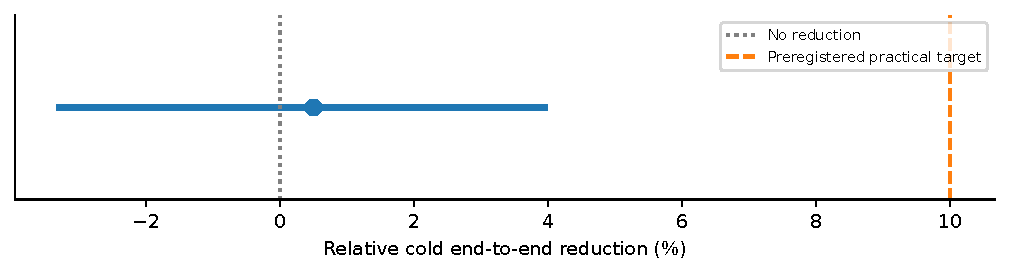
\includegraphics[width=\textwidth]{figures/primary-effect.pdf}
\caption{Primary paired effect and its seed-cluster interval. Positive values indicate reduced cold end-to-end time. The interval includes zero and the point estimate is below the preregistered practical target. Six seed clusters limit generalization beyond this measured environment.}
\end{figure}

\begin{figure}[htbp]\centering
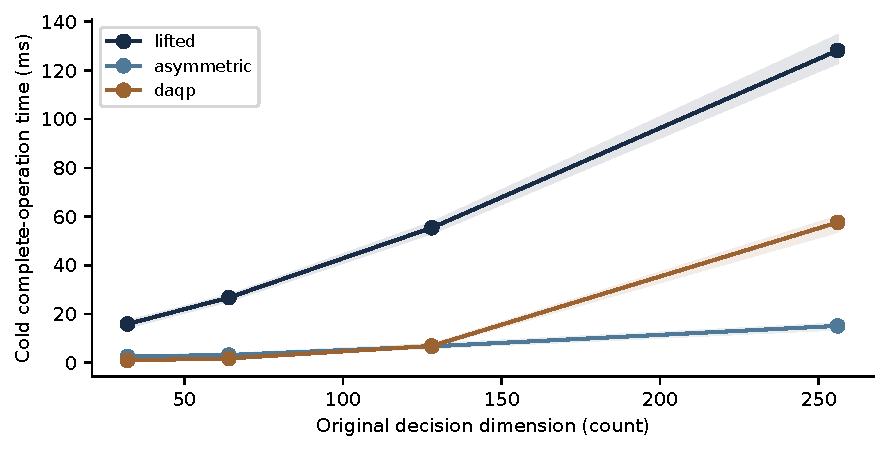
\includegraphics[width=\textwidth]{figures/cold-times.pdf}
\caption{Held-out asymmetric elastic observations at density 0.05. Lines show medians over evaluation seeds and seven measured repetitions; bands show interquartile ranges. Each cold call includes validation and original-space evaluation. Differences between numerical setup and the outer operation prevent inferring an isolated factorization advantage from these curves.}
\end{figure}

\subsection{Controlled conditioning}
The robustness sweep changes only the diagonal objective condition within a seed. All compatible observations remain within the registered objective and hard-row thresholds through condition $10^6$. Figure~\ref{fig:conditioning} shows the maximum normalized objective discrepancy among accepted observations; no unsuccessful observation is replaced with zero. This finite synthetic sweep does not establish reliability for arbitrary row scales, nearly dependent constraints or every semidefinite problem.

\begin{figure}[htbp]\centering
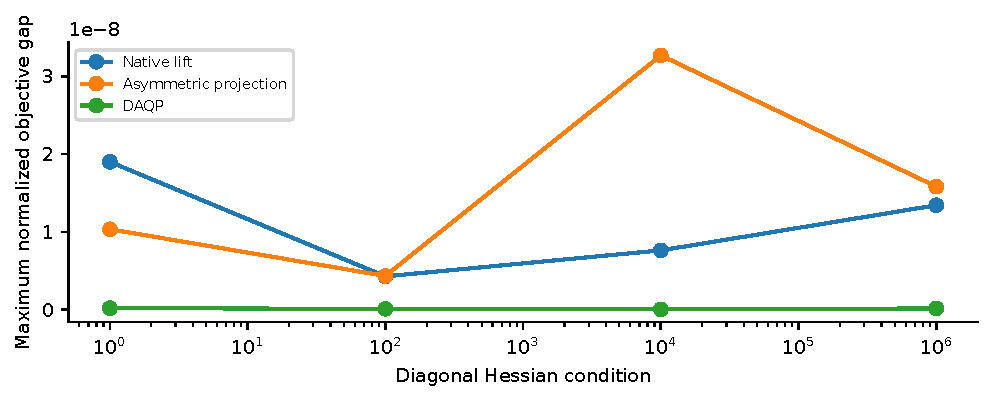
\includegraphics[width=0.9\textwidth]{figures/conditioning.pdf}
\caption{Maximum accepted normalized objective discrepancy in the controlled 32-variable sweep. The original-space acceptance ceiling is $10^{-6}$. Rows, targets, bounds and prices are unchanged within each seed; only the Hessian diagonal condition varies.}\label{fig:conditioning}
\end{figure}

\subsection{Common-trajectory predictive control}
The condensed double integrator has sampling period 0.2~s, horizon 20 and initial state $(1.6,0)$. Its state transition and input vector are
\begin{equation}
F=\begin{pmatrix}1&0.2\\0&1\end{pmatrix},\qquad B=\begin{pmatrix}0.02\\0.2\end{pmatrix}.
\end{equation}
Actuation remains hard in $[-1,1]$~m/s$^2$, while desired position and velocity bands are $\pm0.4$~m and $\pm1.5$~m/s with asymmetric elastic prices. Velocity impulses of $+0.8$ and $-0.6$~m/s occur at frames 8 and 20. An independent high-accuracy lifted controller drives one common plant trajectory. Every compared solver receives those same 32 state inputs, avoiding a confound from diverging controller trajectories.

Three compatible methods each have cold and warm observations at every frame, giving 192 accepted solutions. Generalized symmetric projection contributes 64 incompatible cells. Warm setup is counted once, frame zero has no vector update and later observations include update/solve/evaluation. One observation per frame is descriptive and does not supply a new statistical superiority claim.

\begin{figure}[htbp]\centering
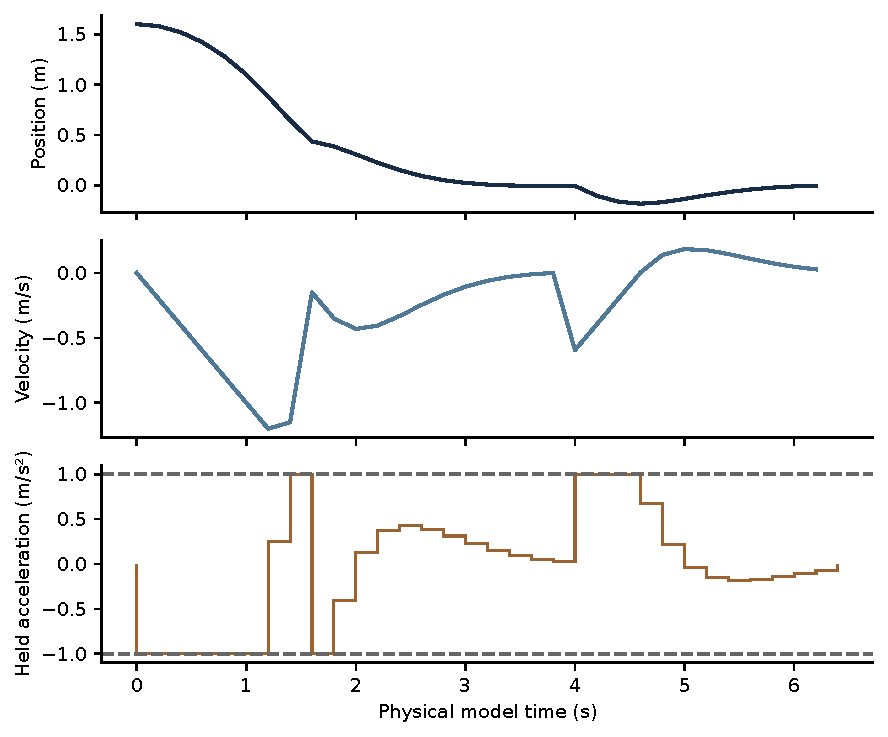
\includegraphics[width=0.96\textwidth]{figures/control-stream.pdf}
\caption{The common oracle-driven plant trajectory. Dotted state boundaries are soft targets; dotted actuator boundaries are hard. Dashed vertical lines mark supplied velocity impulses. Condensed dynamics and bounded oracle actuation define this model example, not a safety certificate for an independent plant.}
\end{figure}

The condensed objective omits a state-dependent constant. Restoring $\tfrac12c^\top Wc$ is necessary before interpreting the predicted physical horizon cost, where $c$ is the uncontrolled state offset. Successive horizon predictions overlap and must not be summed as realized plant cost.

\subsection{Building-energy policies}
The published mixed-cost building input has objective approximately 36.660488. The two authored separable policies have objectives approximately 48.402991 and 42.682180 under their own distinct costs. Those values cannot rank algorithms or policy quality across objectives. Within each policy, compatible native and lifted formulations agree under the external criterion and preserve physical hard constraints.

\begin{figure}[htbp]\centering
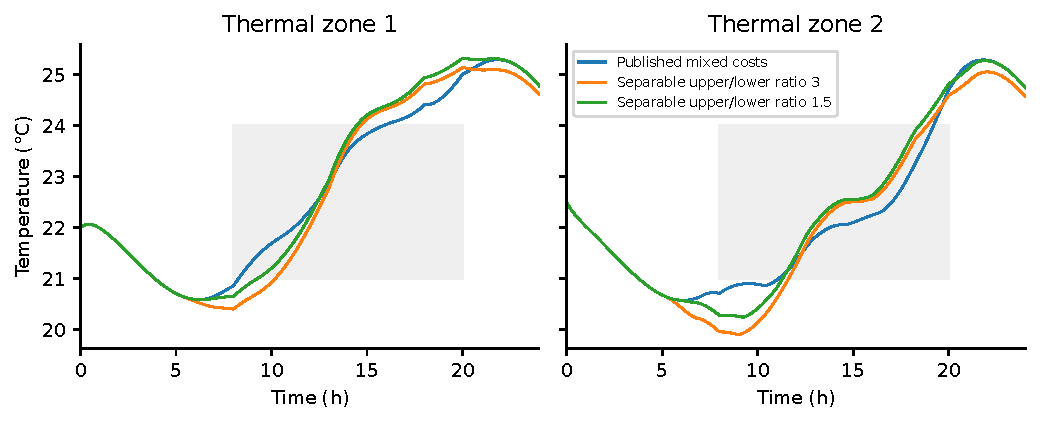
\includegraphics[width=\textwidth]{figures/energy-policies.pdf}
\caption{Thermal predictions under the mixed source policy and two explicitly changed separable policies. The shaded occupied comfort band applies from 8 to 20~h. Curves differ because the optimization prices differ; their shapes are not a solver-accuracy ranking. Source inputs are synthetic and preserve the upstream MIT attribution.}
\end{figure}

\section{Limitations}
The primary result is a negative cold end-to-end comparison on one environment and six evaluation seeds, not an equivalence theorem for runtime. Python validation, reference formulation work, native preparation and the implementation language are included in the operation that was actually measured. A different measurement boundary would answer another question. Isolated numeric factorization and per-method native allocation peaks are unavailable.

The asymmetric native extension is separable and does not implement side-dependent Huber transitions or coupled asymmetric group penalties. The bounded dense references do not cover every convex input accepted by the native sparse path. The fixed FlexQP reconstruction does not reproduce a learned policy or the authors' timing environment. An external hard-optimum interpretation of L1 elasticity additionally requires the appropriate penalty-size conditions.

The control example uses a deterministic known model and shared oracle-driven states. It does not evaluate estimation errors, independent closed-loop policies, actuator dynamics outside the model or safety of deliberately softened state rows. The building input is a published synthetic model, and changing its penalties creates authored variants rather than field evidence.

The scalar proximal derivation and numerical tests do not establish global algorithmic novelty or all adaptive-parameter convergence conditions. Parametric active-set reuse and reduced-system correction already have substantial prior work. A replacement computational proposal would need its own mathematical argument, prior-art assessment and prospective comparison; it cannot inherit a positive interpretation from a failed endpoint.

\section{Conclusions}
Side-specific convex prices make the meaning of a soft interval explicit and can be implemented through a native proximal update while retaining the principal QP dimensions. Independent lifting and compatible published references support original-space numerical agreement over the tested cases. Hard rows, physical units, side violations and backend-specific statuses remain essential parts of that interpretation.

The preregistered cold end-to-end improvement is not established against the faster matched reference. The result limits a performance argument based only on smaller formulations. Reusable workspaces and a common-trajectory control example remain inspectable computational mechanisms, while their practical value requires representative workloads and comparisons with equally capable reference updates.

\section*{Data and code availability}
Source and computational inputs are available at \url{https://github.com/fsantibanezleal/CAOS_SoftQP}; the native package source is \url{https://github.com/fsantibanezleal/CAOS_SoftQP_Engine}. The frozen protocol is \texttt{docs/design/experiments-v1.json}. Complete repeated observations, instance fingerprints, checksums, resource summaries and the common control trajectory are under \texttt{data/derived/experiments/}. The numerical source revision and hashes identify the historical computation independently of later packaging changes. Original per-case x/y, row metadata and objective components are under \texttt{data/derived/softqp/}.

\begin{thebibliography}{9}
\bibitem{osqp} B. Stellato, G. Banjac, P. Goulart, A. Bemporad and S. Boyd. OSQP: an operator splitting solver for quadratic programs. Mathematical Programming Computation, 2020. Solver documentation: \url{https://osqp.org/docs/solver/}.
\bibitem{gsp} R. Schwan, T. Lew and B. Plancher. Efficient ADMM for Soft-Constrained Quadratic Programs via Generalized Slack Projections, 2026. \url{https://arxiv.org/abs/2610.35631}.
\bibitem{daqp} D. Arnstr\"om. DAQP: official soft-constraint formulation and original-scale side-specific weights. \url{https://darnstrom.github.io/daqp/start/advanced/soft}.
\bibitem{flex} A. Oshin and collaborators. Deep FlexQP: Accelerated Nonlinear Programming via Deep Unfolding. ICLR 2026. Fixed-equation source: \url{https://arxiv.org/html/2512.01565v2}.
\bibitem{elasti} D. Morton and collaborators. ElastiQP: An Always-Feasible QP Solver for Constrained Robot Control, 2026. Published implementation: \url{https://github.com/StanfordASL/elastiqp}.
\bibitem{qpoases} qpOASES contributors. qpOASES User's Manual. Online active-set strategy for parametric quadratic programming. \url{https://coin-or.github.io/qpOASES/doc/3.0/manual.pdf}.
\end{thebibliography}
\end{document}
